\renewcommand{\marginalheight}{25pt}
\newcommand{\varphiheight}{38pt}
\newcommand{\fieldheight}{48pt}
\begin{figure}[t]
\centering
    \hspace{-2em}
    \begin{tabular}{p{51pt}@{\hspace{25pt}}m{1pt}c@{\hspace{15pt}}m{1pt}c@{\hspace{15pt}}m{1pt}c}
      \raisebox{23pt}{
      \centering
      \begin{tabular}{c}
        \small$\texttt{Ising}$ \\
        \hspace{5pt}
        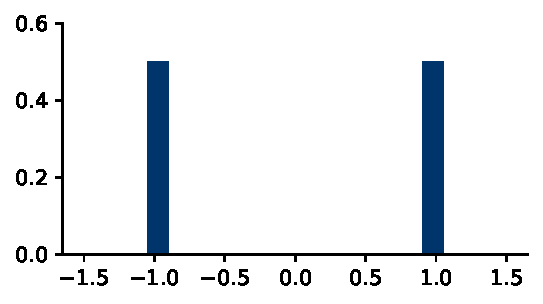
\includegraphics[height=\marginalheight]{figures/task/marginal/ising.pdf}
      \end{tabular}} &
      \raisebox{48pt}{\rotatebox{90}{\tiny $\varphi(a)$}} &
      \raisebox{8pt}{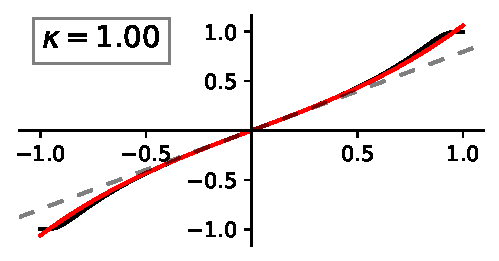
\includegraphics[height=\varphiheight]{figures/theory/varphi/ising.pdf}} &
      \raisebox{44pt}{\rotatebox{90}{\tiny magnitude $w_i$}} &
      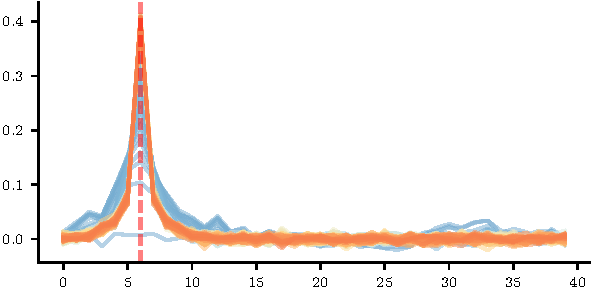
\includegraphics[height=\fieldheight]{figures/theory/rf_evol/ising_neurips.pdf} &
      \raisebox{44pt}{\rotatebox{90}{\tiny magnitude $w_i$}} &
      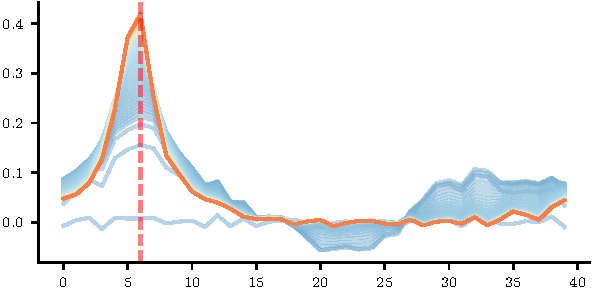
\includegraphics[height=\fieldheight]{figures/theory/rf_sim/ising_kurtosis_neurips.pdf} \\
      \noalign{\vskip -25pt}
      \raisebox{23pt}{
      \begin{tabular}{c}
        \small$\texttt{NLGP}(0.01)$ \\
        \hspace{4pt}
        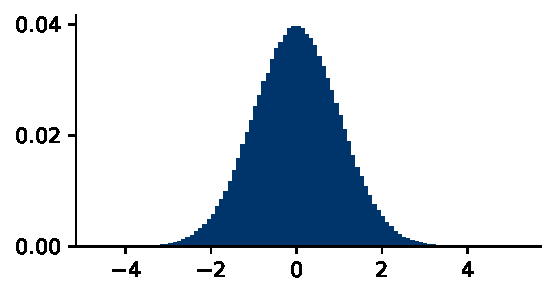
\includegraphics[height=\marginalheight]{figures/task/marginal/gaussian.pdf}
      \end{tabular}} &
      \raisebox{48pt}{\rotatebox{90}{\tiny $\varphi(a)$}} &
      \raisebox{8pt}{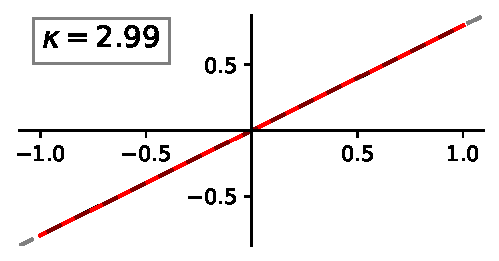
\includegraphics[height=\varphiheight]{figures/theory/varphi/gaussian.pdf}} &
      \raisebox{48pt}{\rotatebox{90}{\tiny magnitude $w_i$}} &
      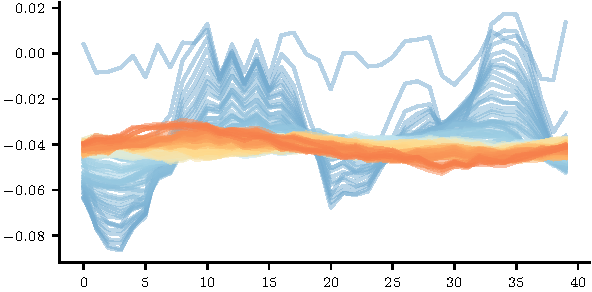
\includegraphics[height=\fieldheight]{figures/theory/rf_evol/gaussian_neurips.pdf} &
      \raisebox{48pt}{\rotatebox{90}{\tiny magnitude $w_i$}} &
      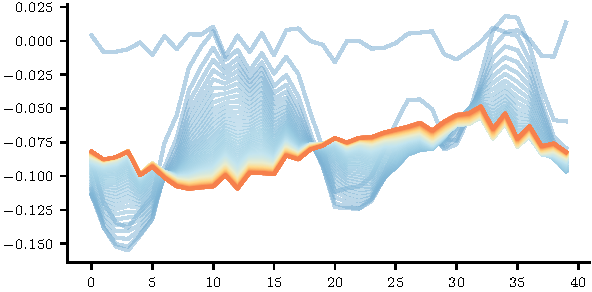
\includegraphics[height=\fieldheight]{figures/theory/rf_sim/gaussian_kurtosis_neurips.pdf} \\
      \noalign{\vskip -25pt}
      \raisebox{23pt}{
      \hspace{.4em}
      \begin{tabular}{c}
        \small $\texttt{Kur}(5)$ \\
        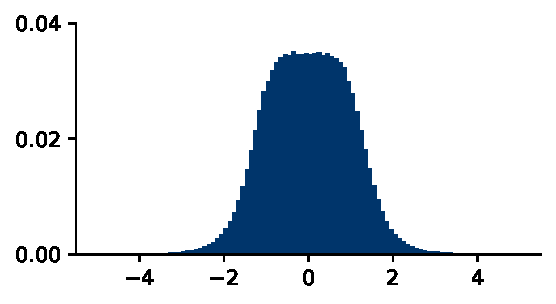
\includegraphics[height=\marginalheight]{figures/task/marginal/alg5.pdf}
      \end{tabular}} &
      \raisebox{48pt}{\rotatebox{90}{\tiny $\varphi(a)$}} &
      \raisebox{8pt}{
      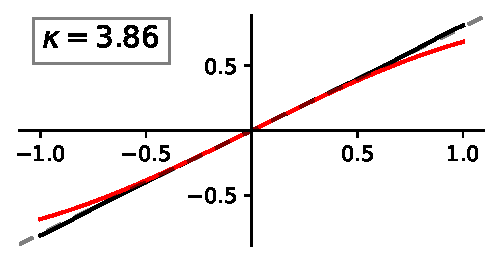
\includegraphics[height=\varphiheight]{figures/theory/varphi/alg5.pdf}
      } &
      \raisebox{44pt}{\rotatebox{90}{\tiny magnitude $w_i$}} &
      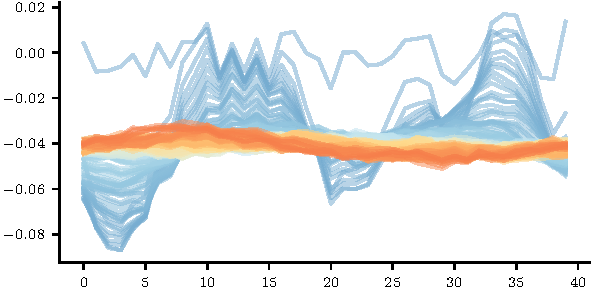
\includegraphics[height=\fieldheight]{figures/theory/rf_evol/alg5_neurips.pdf} &
      \raisebox{44pt}{\rotatebox{90}{\tiny magnitude $w_i$}} &
      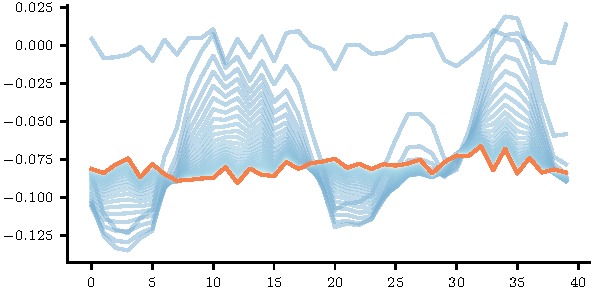
\includegraphics[height=\fieldheight]{figures/theory/rf_sim/alg5_kurtosis_neurips.pdf} \\
      \noalign{\vskip -40pt}
      &&
      \hspace{0pt}\tiny input value $a$ & &
      \hspace{12pt}\tiny dimension $i$ of weight $\mathbf{w}$ & &
      \hspace{12pt}\tiny dimension $i$ of weight $\mathbf{w}$ \\
    \end{tabular}
  \caption{
    从左侧开始,对于与 \cref{fig:task} 中相同的 \texttt{Ising}、\texttt{NLGP} 和 \texttt{Kur} 数据模型:
    边缘分布 $p(X_i)$,
    放大器 $\varphi$(定义见 \cref{lem:gradient_flow})与峰度 $\kappa$,
    以及在其对应数据上训练的单神经元模型(\labelcref{item:single-neuron-model})的模拟感受野演化,
    最后是通过数值积分 \cref{eq:gradient_flow_early} 并将 $\varphi$ 展开为三阶泰勒近似后得到的感受野;
    训练或演化时间由线条颜色表示(蓝色表示早期,红色表示晚期)。
    \emph{详见 \cref{sec:theory-validation} 的阐述。}
  }
  \label{fig:theory}
\end{figure}
